% Figure 1: System Architecture — BDI-LLM Multi-Layer Verification
% Compile with: pdflatex architecture.tex
\documentclass[border=8pt]{standalone}
\usepackage{tikz}
\usetikzlibrary{arrows.meta, positioning, shapes.geometric, fit, calc, backgrounds}
\usepackage{xcolor}

\definecolor{inputcol}{HTML}{E3F2FD}
\definecolor{llmcol}{HTML}{FFF3E0}
\definecolor{structcol}{HTML}{E8F5E9}
\definecolor{symcol}{HTML}{F3E5F5}
\definecolor{repaircol}{HTML}{FBE9E7}
\definecolor{outputcol}{HTML}{E0F7FA}
\definecolor{arrowcol}{HTML}{455A64}
\definecolor{failcol}{HTML}{E53935}
\definecolor{passcol}{HTML}{43A047}

\begin{document}
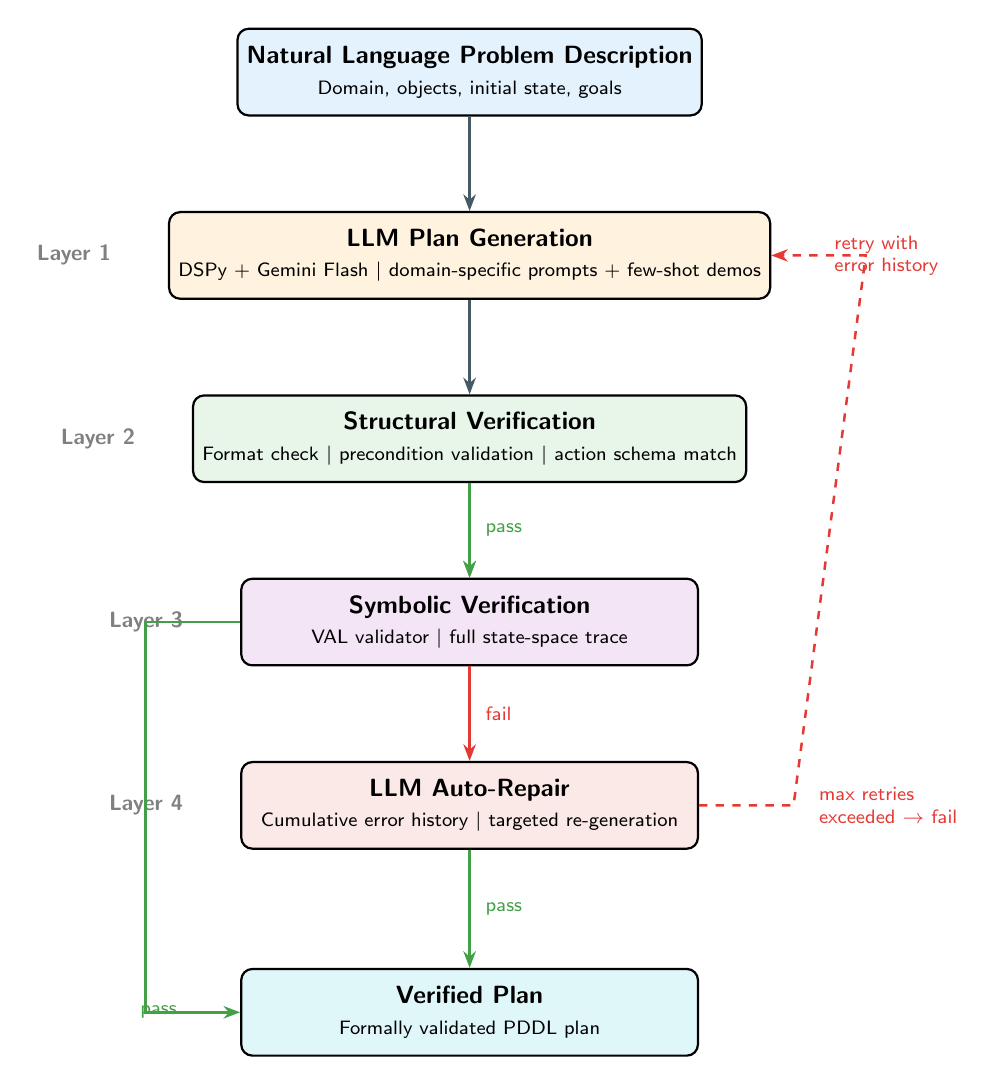
\begin{tikzpicture}[
    node distance=1.2cm and 0.5cm,
    >={Stealth[length=6pt]},
    box/.style={
        draw, rounded corners=4pt, minimum width=5.8cm, minimum height=1.1cm,
        align=center, font=\sffamily\small, line width=0.8pt
    },
    layer/.style={
        font=\sffamily\footnotesize\bfseries, text=gray, anchor=east
    },
    annot/.style={
        font=\sffamily\scriptsize, text=gray!70!black
    },
]

% ── Nodes ──
\node[box, fill=inputcol] (input)
    {\textbf{Natural Language Problem Description}\\
     \scriptsize Domain, objects, initial state, goals};

\node[box, fill=llmcol, below=of input] (llm)
    {\textbf{LLM Plan Generation}\\
     \scriptsize DSPy + Gemini Flash $\mid$ domain-specific prompts + few-shot demos};

\node[box, fill=structcol, below=of llm] (struct)
    {\textbf{Structural Verification}\\
     \scriptsize Format check $\mid$ precondition validation $\mid$ action schema match};

\node[box, fill=symcol, below=of struct] (sym)
    {\textbf{Symbolic Verification}\\
     \scriptsize VAL validator $\mid$ full state-space trace};

\node[box, fill=repaircol, below=of sym] (repair)
    {\textbf{LLM Auto-Repair}\\
     \scriptsize Cumulative error history $\mid$ targeted re-generation};

\node[box, fill=outputcol, below=1.5cm of repair] (output)
    {\textbf{Verified Plan}\\
     \scriptsize Formally validated PDDL plan};

% ── Layer labels ──
\node[layer, left=0.6cm of llm.west]    {Layer 1};
\node[layer, left=0.6cm of struct.west]  {Layer 2};
\node[layer, left=0.6cm of sym.west]     {Layer 3};
\node[layer, left=0.6cm of repair.west]  {Layer 4};

% ── Main flow arrows ──
\draw[->, arrowcol, line width=1pt] (input)  -- (llm);
\draw[->, arrowcol, line width=1pt] (llm)    -- (struct);
\draw[->, arrowcol, line width=1pt] (struct) -- (sym);

% ── Pass / Fail from Structural ──
\draw[->, passcol, line width=0.9pt]
    (struct.south) -- (sym.north)
    node[midway, right=2pt, annot, text=passcol] {pass};

% ── Pass / Fail from Symbolic ──
\coordinate (symR) at ($(sym.east)+(0.4,0)$);
\draw[->, failcol, line width=0.9pt]
    (sym.south) -- (repair.north)
    node[midway, right=2pt, annot, text=failcol] {fail};

% ── Repair feedback loop ──
\coordinate (repairR) at ($(repair.east)+(1.2,0)$);
\coordinate (llmR)    at ($(llm.east)+(1.2,0)$);
\draw[->, failcol, line width=0.9pt, dashed]
    (repair.east) -- (repairR) -- (llmR) -- (llm.east)
    node[pos=0.5, right=2pt, annot, text=failcol, align=left]
    {retry with\\error history};

% ── Repair success → output ──
\draw[->, passcol, line width=1pt]
    (repair.south) -- (output.north)
    node[midway, right=2pt, annot, text=passcol] {pass};

% ── Direct pass from symbolic to output ──
\coordinate (symL) at ($(sym.west)+(-1.2,0)$);
\coordinate (outL) at ($(output.west)+(-1.2,0)$);
\draw[->, passcol, line width=1pt]
    (sym.west) -- (symL) -- (outL) -- (output.west)
    node[pos=0.5, left=2pt, annot, text=passcol] {pass};

% ── Max retries exceeded ──
\node[annot, text=failcol, right=1.4cm of repair.east, anchor=west, align=left]
    (maxretry) {max retries\\exceeded $\rightarrow$ fail};

\end{tikzpicture}
\end{document}
